\pkg{Engine for Likelihood-Free Inference (ELFI)}\footnote{Extended
  documentation can be found
  \href{https://elfi.readthedocs.io/en/latest/}{here}}~\cite{1708.00707}
is a \proglang{Python} package for Likelihood-Free Inference (LFI). We
selected to implemented ROMC in \pkg{ELFI} since it provides
convenient modules for all the fundamental components of a
probabilistic model (e.g.\ prior, simulator, summaries
etc.). Furthermore, \pkg{ELFI} already supports some recently proposed
likelihood-free inference methods, making it straightforward to
perform comparisons between methods. The implementation was officially
added to \pkg{ELFI} in version \pkg{v0.8.0}.

% \subsubsection{Modelling at ELFI}
% \label{sec:modelling}

\pkg{ELFI} models the probabilistic model as a Directed Acyclic Graph
(DAG). This functionality is based on the package \pkg{NetworkX},
which supports general-purpose graphs. In most cases, the structure of
a likelihood-free model follows the pattern of figure~\ref{fig:elfi};
some edges connect the prior distributions to the simulator, the
simulator is connected to the summary statistics that, in turn, lead
to the output node. Samples can be obtained from all nodes through
sequential (ancestral) sampling. \pkg{ELFI} automatically considers as
parameters of interest, i.e. those we try to infer a posterior
distribution, as the ones defined through the \code{elfi.Prior}
class. Finally, the observations are passed to the appropriate node
through the argument
\code{observed}.

\begin{figure}[ht]
    \begin{center}
      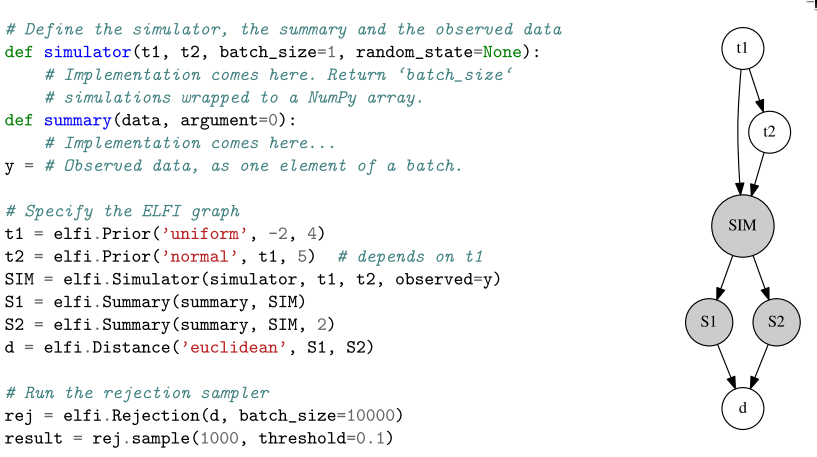
\includegraphics[width=0.8\textwidth]{./latex_files/images/chapter2/elfi.png}
    \end{center}
    \caption[Baseline example for creating an \pkg{ELFI} model]{Baseline example for creating an \pkg{ELFI} model. Image taken from \cite{1708.00707}}
    \label{fig:elfi}
\end{figure}

% \subsubsection{Inference at ELFI}
% \label{sec:inference-methods}

All inference methods in \pkg{ELFI} share the following rules;

\begin{itemize}
\item they follow the signature \code{elfi.<Class name>(<output node>,
    *arg)}; the initial argument is the output node model and the rest
  of the arguments are hyper-parameters of the method.
\item they provide a central sampling functionality, which in most
  cases is named \\ \code{<method_name>.sample()}.
\end{itemize}
